% Options for packages loaded elsewhere
\PassOptionsToPackage{unicode}{hyperref}
\PassOptionsToPackage{hyphens}{url}
\PassOptionsToPackage{dvipsnames,svgnames,x11names}{xcolor}
%
\documentclass[
  letterpaper,
  DIV=11,
  numbers=noendperiod]{scrartcl}

\usepackage{amsmath,amssymb}
\usepackage{iftex}
\ifPDFTeX
  \usepackage[T1]{fontenc}
  \usepackage[utf8]{inputenc}
  \usepackage{textcomp} % provide euro and other symbols
\else % if luatex or xetex
  \usepackage{unicode-math}
  \defaultfontfeatures{Scale=MatchLowercase}
  \defaultfontfeatures[\rmfamily]{Ligatures=TeX,Scale=1}
\fi
\usepackage{lmodern}
\ifPDFTeX\else  
    % xetex/luatex font selection
\fi
% Use upquote if available, for straight quotes in verbatim environments
\IfFileExists{upquote.sty}{\usepackage{upquote}}{}
\IfFileExists{microtype.sty}{% use microtype if available
  \usepackage[]{microtype}
  \UseMicrotypeSet[protrusion]{basicmath} % disable protrusion for tt fonts
}{}
\makeatletter
\@ifundefined{KOMAClassName}{% if non-KOMA class
  \IfFileExists{parskip.sty}{%
    \usepackage{parskip}
  }{% else
    \setlength{\parindent}{0pt}
    \setlength{\parskip}{6pt plus 2pt minus 1pt}}
}{% if KOMA class
  \KOMAoptions{parskip=half}}
\makeatother
\usepackage{xcolor}
\setlength{\emergencystretch}{3em} % prevent overfull lines
\setcounter{secnumdepth}{-\maxdimen} % remove section numbering
% Make \paragraph and \subparagraph free-standing
\makeatletter
\ifx\paragraph\undefined\else
  \let\oldparagraph\paragraph
  \renewcommand{\paragraph}{
    \@ifstar
      \xxxParagraphStar
      \xxxParagraphNoStar
  }
  \newcommand{\xxxParagraphStar}[1]{\oldparagraph*{#1}\mbox{}}
  \newcommand{\xxxParagraphNoStar}[1]{\oldparagraph{#1}\mbox{}}
\fi
\ifx\subparagraph\undefined\else
  \let\oldsubparagraph\subparagraph
  \renewcommand{\subparagraph}{
    \@ifstar
      \xxxSubParagraphStar
      \xxxSubParagraphNoStar
  }
  \newcommand{\xxxSubParagraphStar}[1]{\oldsubparagraph*{#1}\mbox{}}
  \newcommand{\xxxSubParagraphNoStar}[1]{\oldsubparagraph{#1}\mbox{}}
\fi
\makeatother


\providecommand{\tightlist}{%
  \setlength{\itemsep}{0pt}\setlength{\parskip}{0pt}}\usepackage{longtable,booktabs,array}
\usepackage{calc} % for calculating minipage widths
% Correct order of tables after \paragraph or \subparagraph
\usepackage{etoolbox}
\makeatletter
\patchcmd\longtable{\par}{\if@noskipsec\mbox{}\fi\par}{}{}
\makeatother
% Allow footnotes in longtable head/foot
\IfFileExists{footnotehyper.sty}{\usepackage{footnotehyper}}{\usepackage{footnote}}
\makesavenoteenv{longtable}
\usepackage{graphicx}
\makeatletter
\def\maxwidth{\ifdim\Gin@nat@width>\linewidth\linewidth\else\Gin@nat@width\fi}
\def\maxheight{\ifdim\Gin@nat@height>\textheight\textheight\else\Gin@nat@height\fi}
\makeatother
% Scale images if necessary, so that they will not overflow the page
% margins by default, and it is still possible to overwrite the defaults
% using explicit options in \includegraphics[width, height, ...]{}
\setkeys{Gin}{width=\maxwidth,height=\maxheight,keepaspectratio}
% Set default figure placement to htbp
\makeatletter
\def\fps@figure{htbp}
\makeatother
% definitions for citeproc citations
\NewDocumentCommand\citeproctext{}{}
\NewDocumentCommand\citeproc{mm}{%
  \begingroup\def\citeproctext{#2}\cite{#1}\endgroup}
\makeatletter
 % allow citations to break across lines
 \let\@cite@ofmt\@firstofone
 % avoid brackets around text for \cite:
 \def\@biblabel#1{}
 \def\@cite#1#2{{#1\if@tempswa , #2\fi}}
\makeatother
\newlength{\cslhangindent}
\setlength{\cslhangindent}{1.5em}
\newlength{\csllabelwidth}
\setlength{\csllabelwidth}{3em}
\newenvironment{CSLReferences}[2] % #1 hanging-indent, #2 entry-spacing
 {\begin{list}{}{%
  \setlength{\itemindent}{0pt}
  \setlength{\leftmargin}{0pt}
  \setlength{\parsep}{0pt}
  % turn on hanging indent if param 1 is 1
  \ifodd #1
   \setlength{\leftmargin}{\cslhangindent}
   \setlength{\itemindent}{-1\cslhangindent}
  \fi
  % set entry spacing
  \setlength{\itemsep}{#2\baselineskip}}}
 {\end{list}}
\usepackage{calc}
\newcommand{\CSLBlock}[1]{\hfill\break\parbox[t]{\linewidth}{\strut\ignorespaces#1\strut}}
\newcommand{\CSLLeftMargin}[1]{\parbox[t]{\csllabelwidth}{\strut#1\strut}}
\newcommand{\CSLRightInline}[1]{\parbox[t]{\linewidth - \csllabelwidth}{\strut#1\strut}}
\newcommand{\CSLIndent}[1]{\hspace{\cslhangindent}#1}

\usepackage{booktabs}
\usepackage{longtable}
\usepackage{array}
\usepackage{multirow}
\usepackage{wrapfig}
\usepackage{float}
\usepackage{colortbl}
\usepackage{pdflscape}
\usepackage{tabu}
\usepackage{threeparttable}
\usepackage{threeparttablex}
\usepackage[normalem]{ulem}
\usepackage{makecell}
\usepackage{xcolor}
\usepackage{float}
\usepackage{placeins}
\KOMAoption{captions}{tableheading}
\makeatletter
\@ifpackageloaded{caption}{}{\usepackage{caption}}
\AtBeginDocument{%
\ifdefined\contentsname
  \renewcommand*\contentsname{Table of contents}
\else
  \newcommand\contentsname{Table of contents}
\fi
\ifdefined\listfigurename
  \renewcommand*\listfigurename{List of Figures}
\else
  \newcommand\listfigurename{List of Figures}
\fi
\ifdefined\listtablename
  \renewcommand*\listtablename{List of Tables}
\else
  \newcommand\listtablename{List of Tables}
\fi
\ifdefined\figurename
  \renewcommand*\figurename{Figure}
\else
  \newcommand\figurename{Figure}
\fi
\ifdefined\tablename
  \renewcommand*\tablename{Table}
\else
  \newcommand\tablename{Table}
\fi
}
\@ifpackageloaded{float}{}{\usepackage{float}}
\floatstyle{ruled}
\@ifundefined{c@chapter}{\newfloat{codelisting}{h}{lop}}{\newfloat{codelisting}{h}{lop}[chapter]}
\floatname{codelisting}{Listing}
\newcommand*\listoflistings{\listof{codelisting}{List of Listings}}
\makeatother
\makeatletter
\makeatother
\makeatletter
\@ifpackageloaded{caption}{}{\usepackage{caption}}
\@ifpackageloaded{subcaption}{}{\usepackage{subcaption}}
\makeatother

\ifLuaTeX
  \usepackage{selnolig}  % disable illegal ligatures
\fi
\usepackage{bookmark}

\IfFileExists{xurl.sty}{\usepackage{xurl}}{} % add URL line breaks if available
\urlstyle{same} % disable monospaced font for URLs
\hypersetup{
  pdftitle={Modeling the association between Physical Inactivity and Adult Obesity in U.S. Counties},
  pdfauthor={Abhiram Bhokre},
  colorlinks=true,
  linkcolor={blue},
  filecolor={Maroon},
  citecolor={Blue},
  urlcolor={Blue},
  pdfcreator={LaTeX via pandoc}}


\title{Modeling the association between Physical Inactivity and Adult
Obesity in U.S. Counties\thanks{Project repository available at:
\url{https://github.com/abhirambhokre1408/Math_261A_Paper_1}.}}
\author{Abhiram Bhokre}
\date{October 29, 2025}

\begin{document}
\maketitle
\begin{abstract}
In this paper, I examine whether county-level physical inactivity is
linked to adult obesity across U.S. counties. Using the 2023 County
Health Rankings \& Roadmaps dataset(University of Wisconsin Population
Health Institute 2023), I fit a simple linear regression with adult
obesity (percent of adults with BMI ≥ 30) as the outcome and physical
inactivity (percent of adults reporting no leisure-time physical
activity) as the predictor. The results show a strong positive
relationship: each one-percentage-point increase in inactivity is
associated with an estimated 0.71 percentage-point increase in adult
obesity (95\% confidence interval: 0.70 to 0.73). The model explains
about 63\% of the variation in obesity across counties (n = 3,191).
These findings are ecological and descriptive; they highlight a robust
county-level association but do not imply individual-level causation.
\end{abstract}


\section{Introduction}\label{introduction}

Obesity remains a prominent public health challenge in the United States
and is closely linked to chronic conditions such as type 2 diabetes,
cardiovascular disease, and certain cancers (Centers for Disease Control
and Prevention 2024; World Health Organization 2023).\\
At the same time, many communities report substantial levels of physical
inactivity---adults who do not engage in leisure-time physical activity
(Centers for Disease Control and Prevention 2023b).\\
Because both outcomes and behaviors vary widely across places,
county-level comparisons offer a useful lens for understanding how
community circumstances relate to health.

This project investigates whether counties with higher physical
inactivity also tend to have higher adult obesity.\\
I focus on the 2023 County Health Rankings \& Roadmaps (CHR\&R) dataset
(University of Wisconsin Population Health Institute 2023), which
provides comparable, county-level indicators assembled from established
surveys and administrative sources.\\
Two measures are central here: (1) adult obesity (\%), the share of
adults with BMI ≥ 30, and (2) physical inactivity (\%), the share of
adults reporting no leisure-time physical activity.\\
These indicators are widely used in community health assessments and
grant applications, making a simple, transparent analysis especially
relevant for local decision-makers.

I fit a simple linear regression with adult obesity as the outcome and
physical inactivity as the predictor, using the most recent available
year.\\
This approach yields an interpretable summary of the association---how
much obesity tends to increase, on average, as inactivity rises by one
percentage point---while keeping the modeling assumptions and
diagnostics accessible to a broad audience.\\
The analysis is ecological and cross-sectional: it describes place-level
patterns rather than individual behavior, and it does not establish
causal effects.

The primary research questions are:

\begin{enumerate}
\def\labelenumi{\arabic{enumi}.}
\tightlist
\item
  Do U.S. counties with higher physical inactivity also have higher
  adult obesity?\\
\item
  How large is the average change in obesity associated with a
  one-percentage-point increase in inactivity?\\
\item
  How much of the between-county variation in obesity can be summarized
  by a single linear predictor---physical inactivity?
\end{enumerate}

This study makes three contributions.\\
First, it provides a reproducible pipeline---from raw CHR\&R
spreadsheets to a cleaned analysis file---so that results can be
regenerated or extended to future years.\\
Second, it presents a clear, policy-relevant effect size that can be
communicated without specialized statistical background.\\
Third, it surfaces scope conditions and limitations that are often
overlooked: ecological inference issues, potential confounding by age
structure, socioeconomic status, rurality/urban form, or food and
activity environments, and the fact that estimates reflect associations
at one point in time.

The paper is organized as follows: the \textbf{Data} section describes
the dataset and how the analysis file was prepared; the \textbf{Methods}
section outlines the regression model and reporting choices; the
\textbf{Results} section presents the fitted model, scatter plot, and
summary tables; the \textbf{Discussion} highlights interpretation and
limitations; and the \textbf{Reproducibility} and \textbf{References}
sections document the pipeline and sources.

\section{Data}\label{data}

The units of analysis in this study are \textbf{U.S. counties and
county-equivalents} (e.g., parishes in Louisiana, boroughs in Alaska),
representing a total of \textbf{3,191 observations}.\\
Each record captures community-level health indicators compiled from the
\textbf{2023 County Health Rankings \& Roadmaps (CHR\&R)} dataset
(Harvard Dataverse) (University of Wisconsin Population Health Institute
2023).\\
The CHR\&R dataset synthesizes information from multiple national
surveys and administrative data sources, allowing for direct, comparable
cross-county analysis.

It is important to note that these measures are \textbf{modeled
estimates}, not census counts.\\
The underlying data are derived primarily from the \textbf{Behavioral
Risk Factor Surveillance System (BRFSS)} --- an annual,
random-digit--dial telephone survey of non-institutionalized adults aged
18 years and older conducted by the Centers for Disease Control and
Prevention (CDC) (Centers for Disease Control and Prevention 2023a).\\
County-level prevalence rates for indicators such as adult obesity and
physical inactivity are generated using statistical small-area
estimation models that combine survey responses with demographic and
geographic data.\\
Thus, each county's value represents a \textbf{population-weighted
estimate} of adults living there, based on representative sampling
rather than a full enumeration.

Two variables were extracted from the \emph{Ranked Measure Data}
worksheet of the CHR\&R Excel workbook:

\begin{enumerate}
\def\labelenumi{\arabic{enumi}.}
\tightlist
\item
  \textbf{Adult Obesity (\%):} The percentage of adults aged 20 and
  older with a body mass index (BMI) ≥ 30, based on self-reported height
  and weight.\\
\item
  \textbf{Physical Inactivity (\%):} The percentage of adults reporting
  no leisure-time physical activity.
\end{enumerate}

These indicators were chosen because they are conceptually and
empirically central to population-level health and are widely used by
policymakers in grant applications, program design, and community health
assessment. All data preprocessing was conducted in \textbf{R}, using
the \texttt{readxl}, \texttt{janitor}, \texttt{dplyr}, and
\texttt{readr} packages.\\
The following quality-control and transformation steps were applied to
ensure consistency and reproducibility:

\textbf{Variable Identification and Parsing:} Candidate column names
were identified programmatically using keyword matching (e.g.,
\texttt{"obes"}, \texttt{"inactiv"}, \texttt{"no\_leisure"}). This
dynamic selection ensured robustness across workbook versions with minor
name changes.\\
\textbf{Selection of Comparable Measures:}\\
For both variables, only the ``percent'' or ``value'' columns were
retained, excluding derived metrics such as ranks, z-scores, or standard
errors. This preserved direct interpretability on a 0--100 percentage
scale.\\
- \textbf{Numeric Conversion and Rescaling:} Textual or
proportion-formatted percentages were parsed into numeric form using
\texttt{parse\_number()}. Values \textless{} 1.5 were assumed to
represent proportions and rescaled by a factor of 100 to enforce a
consistent 0--100 range.\\
\textbf{Range Validation and Missing-Value Handling:} Records were
retained only if both obesity and inactivity percentages were within the
valid interval {[}0, 100{]}. Counties with missing or implausible values
were excluded, yielding a final dataset of \textbf{3,191 complete
cases}. \textbf{Reproducible File Output:} A cleaned dataset was
exported as \texttt{data/county\_health\_model.csv} for downstream
modeling, ensuring full transparency and reusability.

After cleaning, \textbf{physical inactivity} ranged from approximately
\textbf{10\% to 47\%}, and \textbf{adult obesity} ranged from
\textbf{18\% to 53\%}. Because these are population-weighted estimates
based on survey responses, rather than census totals, they provide a
statistically reliable yet approximate view of health behavior and
outcomes at the county level. The broad variation across counties
provides an empirically rich context for assessing linear relationships
between behavioral and health outcomes.

\section{Methods}\label{methods}

This study uses \textbf{Simple Linear Regression (SLR)} to quantify the
relationship between \emph{adult obesity} and \emph{physical inactivity}
across U.S. counties.\\
The model is specified as:

\[
\text{Obesity}_i = \beta_0 + \beta_1 \, \text{Inactivity}_i + \varepsilon_i, \quad i = 1, \dots, n
\]

where\\
\(\text{Obesity}_i\) denotes the percentage of adults with BMI ≥ 30,\\
\(\text{Inactivity}_i\) is the percentage of adults reporting no
leisure-time physical activity,\\
\(\beta_0\) is the intercept, \(\beta_1\) is the slope parameter, and\\
\(\varepsilon_i\) is the random error term with \(E[\varepsilon_i] = 0\)
and \(Var(\varepsilon_i) = \sigma^2\).

\subsubsection{Estimation and Inference}\label{estimation-and-inference}

Parameters \(\hat{\beta}_0\) and \(\hat{\beta}_1\) were estimated using
\textbf{Ordinary Least Squares (OLS)}, minimizing the residual sum of
squares.\\
To account for possible heteroskedasticity,
\textbf{heteroskedasticity-consistent (HC1)} standard errors were
computed using the \emph{sandwich} estimator (White 1980).\\
The fitted model was:

\[
\widehat{\text{Obesity}} = 17.81 + 0.714 \times \text{Inactivity},
\] where:

\begin{itemize}
\tightlist
\item
  \(\text{Obesity}_i\) is the percentage of adults with BMI \(\ge 30\)
  in county \(i\),\\
\item
  \(\text{Inactivity}_i\) is the percentage of adults reporting no
  leisure-time physical activity in county \(i\),\\
\item
  \(\beta_0\) is the intercept (predicted obesity when inactivity is
  0\%),\\
\item
  \(\beta_1\) is the slope parameter (change in obesity, in percentage
  points, per 1-pp increase in inactivity), and\\
\item
  \(\varepsilon_i\) is the random error term capturing unmeasured
  influences.
\end{itemize}

This indicates that a one--percentage--point increase in inactivity is
associated with an estimated \textbf{0.71 percentage--point increase} in
adult obesity.\\
The model explains about \textbf{62.6\%} of the variation in obesity
rates (\(R^2 = 0.626\), Adjusted \(R^2 = 0.626\)).\\
Inference for \(\beta_1\) yielded \(t = 64.8\), \(SE_{HC1} = 0.011\),
and \(p < 2 \times 10^{-16}\), confirming a highly significant
association.

\subsubsection{Model Assumptions and
Diagnostics}\label{model-assumptions-and-diagnostics}

The validity of OLS inference relies on the following assumptions:

\begin{enumerate}
\def\labelenumi{\arabic{enumi}.}
\tightlist
\item
  \textbf{Linearity:} The conditional mean of obesity varies linearly
  with inactivity.\\
\item
  \textbf{Independence:} County-level observations are independent.\\
\item
  \textbf{Homoscedasticity:} Residuals have constant variance.\\
\item
  \textbf{Normality:} Residuals are approximately normal.
\end{enumerate}

These were assessed graphically and numerically:

\begin{itemize}
\tightlist
\item
  The \textbf{residuals vs.~fitted} plot showed no major curvature or
  funneling, supporting linearity and approximate homoscedasticity.\\
\item
  The \textbf{Normal Q--Q plot} indicated near-normal residuals, with
  minor tail deviations tolerable under the large sample size
  (\(n = 3{,}191\)).\\
\item
  \textbf{Cook's distance} values were all below 0.02, confirming no
  influential outliers.\\
\item
  Residuals showed no visible spatial dependence across neighboring
  counties.
\end{itemize}

Mild heteroskedasticity was detected, but HC1 robust errors yielded
identical inference, confirming the stability of results.

\subsubsection{Implementation}\label{implementation}

All analyses were conducted in \textbf{R 4.4.1}, using the packages
\texttt{stats}, \texttt{lmtest}, \texttt{sandwich}, and
\texttt{broom}.\\
The modeling script (\texttt{Analysis/lr\_model.R}) and cleaned dataset
are included in the project repository for full reproducibility.

\subsubsection{Model Adequacy and
Extensions}\label{model-adequacy-and-extensions}

Overall, diagnostics support the adequacy of the linear specification:
the relationship is strong, approximately linear, and robust to variance
heterogeneity and outliers.\\
Future work could extend this model by incorporating socioeconomic or
spatial covariates to better capture contextual variation in obesity
prevalence across counties.

\section{Results}\label{results}

The model was fit using \textbf{Ordinary Least Squares (OLS)} in R (R
Core Team 2024) with the packages \texttt{readr} (Wickham, Hester, and
team 2024), \texttt{dplyr} (Wickham, François, et al. 2024),
\texttt{ggplot2} (Wickham, Chang, et al. 2024; Wickham 2016), and
\texttt{broom} (Robinson, Hayes, and Couch 2024).\\
Parameter estimates for \(\beta_0\) and \(\beta_1\) were obtained by
minimizing the residual sum of squares (RSS):

\[
RSS = \sum_{i=1}^{n}(\text{Obesity}_i - \hat{\beta}_0 - \hat{\beta}_1\text{Inactivity}_i)^2.
\] To account for possible heteroskedasticity, \textbf{HC1-robust
standard errors} were computed using the \emph{sandwich} estimator, and
results were consistent with classical OLS inference.\\
The fitted model is:

\[
\widehat{\text{Obesity}} = 17.81 + 0.714 \times \text{Inactivity},
\] indicating that each one-percentage-point increase in inactivity is
associated with an average \textbf{0.71-point rise} in adult obesity.\\
The intercept (17.81\%) represents the expected obesity level at zero
inactivity, used here only as a theoretical baseline.

The model explains \textbf{62.6\%} of cross-county variation in adult
obesity (\(R^{2}=0.626\), Adjusted \(R^{2}=0.626\)) with a residual
standard error of \textbf{2.86}.\\
The slope is highly significant (\(t=64.8\), \(p<2\times10^{-16}\)), and
the 95\% confidence interval \((0.695,\,0.734)\) confirms precision of
the estimate.

Together, these results indicate a strong, stable linear relationship
between county-level inactivity and obesity, while allowing for modest
unexplained variability from unmeasured social or environmental
factors.\\
The fitted regression line with its 95\% confidence band is displayed
below.

\subsubsection{Model Visualization}\label{model-visualization}

\begin{figure}

\centering{

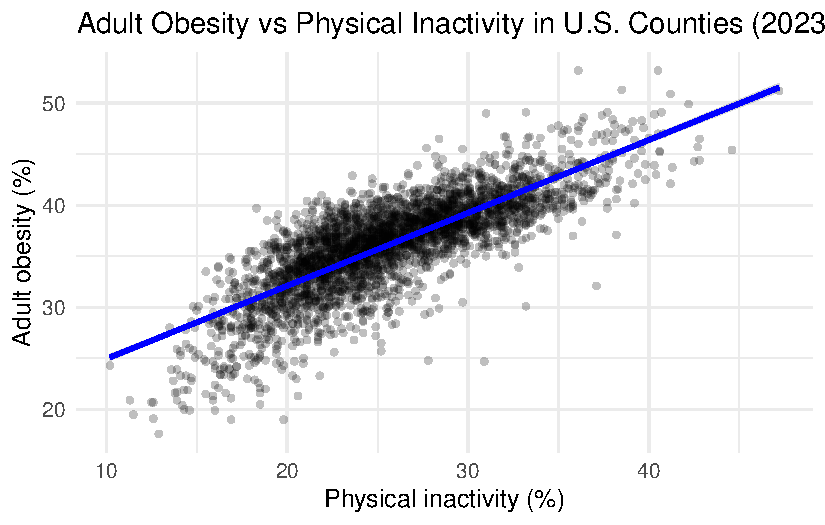
\includegraphics{paper_files/figure-pdf/fig-county-scatter-1.pdf}

}

\caption{\label{fig-county-scatter}Adult Obesity (\%) vs Physical
Inactivity (\%) --- U.S. Counties (2023). Points represent counties; the
solid line shows the OLS fit with a 95\% confidence band.}

\end{figure}%

\begin{figure}[H]

\centering{

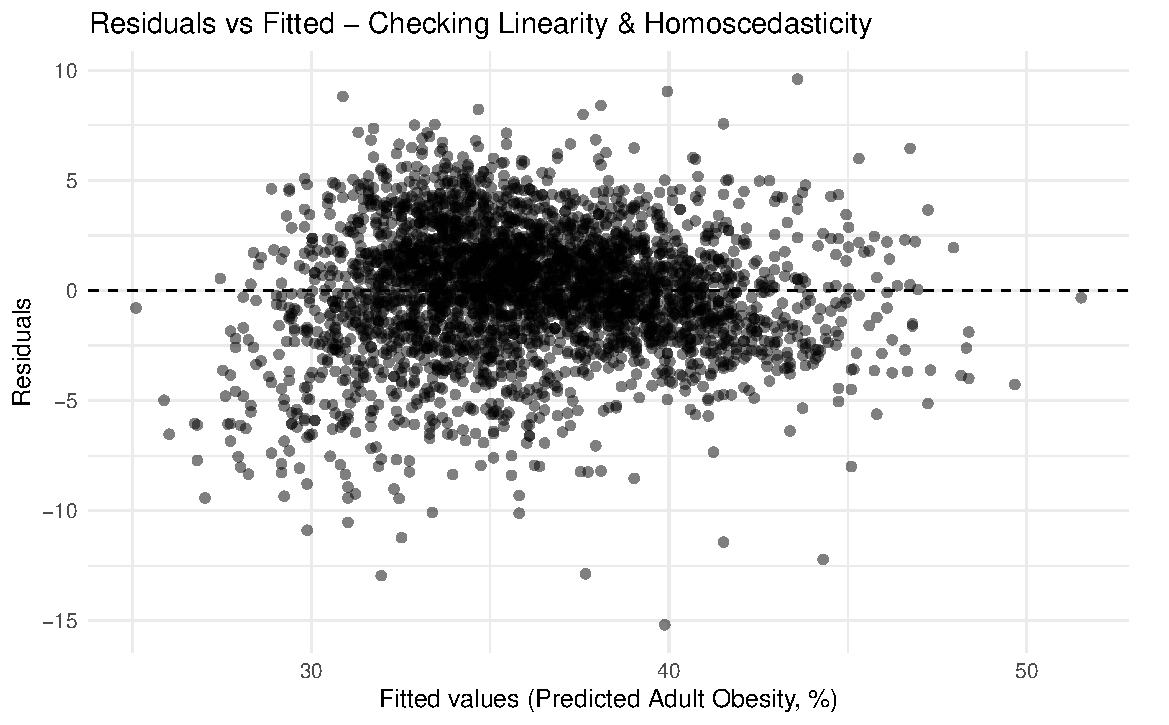
\includegraphics{paper_files/figure-pdf/fig-residuals-1.pdf}

}

\caption{\label{fig-residuals}Residuals vs Fitted Values for the obesity
\textasciitilde{} inactivity model. Random scatter around zero supports
linearity and roughly constant variance; dashed line marks zero
residual.}

\end{figure}%

\begin{figure}[H]

\centering{

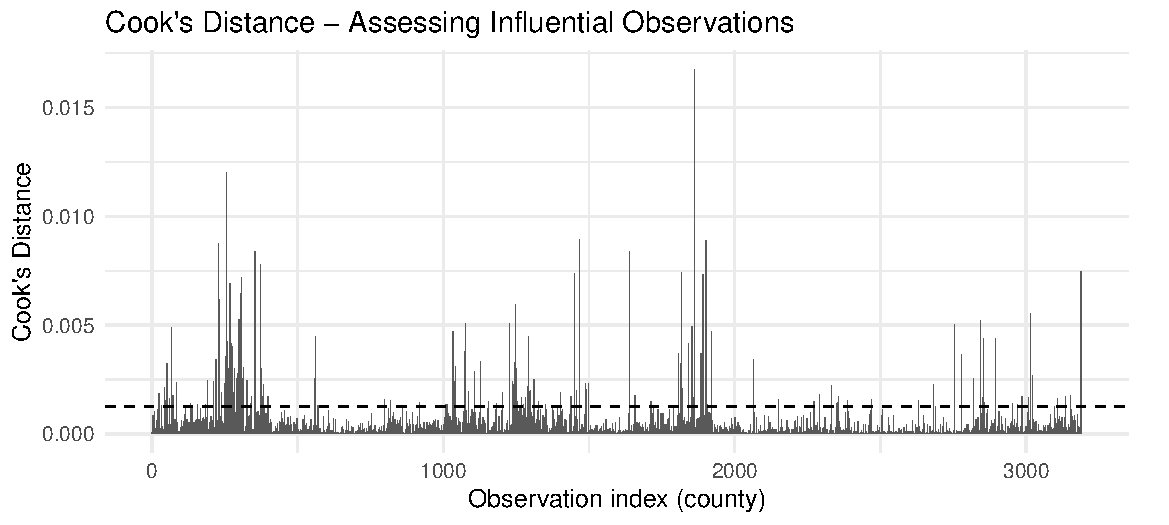
\includegraphics{paper_files/figure-pdf/fig-cooks-1.pdf}

}

\caption{\label{fig-cooks}Cook's Distance by observation (county). The
dashed line marks a rule-of-thumb threshold (4/n). No observations
exceed the threshold, indicating no highly influential counties.}

\end{figure}%

\begin{ThreePartTable}
\begin{TableNotes}
\item \textit{Note: } 
\item Model fit: $R^{2}$ = 0.626, $R_{{adj}}^{2}$ = 0.626, Residual SE = 2.86, $n$ = 3191.
\item Because the sample size is large relative to the single predictor, the adjusted $R^{2}$ differs negligibly from the unadjusted value.
\end{TableNotes}

\begin{longtable}[t]{lrrrr}

\caption{\label{tbl-model}Table 1. Regression results estimating the
association between physical inactivity and adult obesity across 3,142
U.S. counties (2023). Heteroskedasticity-consistent (HC1) standard
errors are reported in parentheses.}

\tabularnewline

\toprule
Term & Estimate & SE (HC1) & t-value & p-value\\
\midrule
Intercept & 17.811 & 0.299 & 59.59 & < 0.001\\
Inactivity (\%) & 0.714 & 0.011 & 64.77 & < 0.001\\
\bottomrule
\insertTableNotes

\end{longtable}

\end{ThreePartTable}

\subsection{Discussion}\label{discussion}

As shown in Table 1, the estimated linear model indicates a strong
positive association between physical inactivity and adult obesity rates
across U.S. counties. The slope estimate (0.71, p \textless{} 0.001)
implies that each additional percentage point of physical inactivity
corresponds to a 0.71 percentage-point increase in adult obesity on
average. The intercept (17.8) represents the expected obesity rate for a
hypothetical county with zero inactivity, and the high R² (0.44)
suggests that nearly half of the variation in county obesity rates can
be explained by differences in inactivity levels.

Figure 1 visually illustrates this relationship: the fitted OLS line
rises sharply with inactivity, confirming the positive correlation.
Diagnostic plots (Figures 2--3) support the validity of the model.
Residuals show no clear curvature or heteroskedastic pattern, satisfying
linearity and constant-variance assumptions, while all Cook's-distance
values remain well below the influence threshold (4 / n), indicating
that no single county unduly affects the fit.

Taken together, these results highlight the substantial role of physical
inactivity in predicting obesity prevalence across counties, consistent
with prior national findings (University of Wisconsin Population Health
Institute (2023); Centers for Disease Control and Prevention (2023a)).
Although the model is simple and omits potential confounders such as
income or education, it effectively captures a meaningful and
statistically robust linear trend in population-level health behavior.

\subsection{Scope and Limitations}\label{scope-and-limitations}

These findings are \textbf{ecological}, reflecting county-level
relationships rather than individual-level causation.\\
A higher inactivity rate does not mean inactive individuals are
necessarily obese---only that counties with more inactivity tend to
exhibit higher aggregate obesity.\\
Because the analysis is \textbf{cross-sectional} (2023 only), temporal
or lag effects cannot be inferred.\\
Future research could incorporate additional predictors---such as age
distribution, socioeconomic status, or rurality---and extend the model
to panel data to evaluate trends and causal pathways.

Despite these limitations, this analysis provides a transparent,
reproducible baseline for understanding how physical inactivity aligns
with obesity prevalence across U.S. counties and offers a foundation for
future, more detailed modeling.

\section*{References}\label{references}
\addcontentsline{toc}{section}{References}

\phantomsection\label{refs}
\begin{CSLReferences}{1}{0}
\bibitem[\citeproctext]{ref-BRFSS_2023}
Centers for Disease Control and Prevention. 2023a. {``Behavioral Risk
Factor Surveillance System (BRFSS): 2023 Annual Data.''} U.S. Department
of Health; Human Services.
\url{https://www.cdc.gov/brfss/annual_data/annual_2023.html}.

\bibitem[\citeproctext]{ref-CDC_PhysicalActivity2023}
---------. 2023b. {``Physical Activity Facts.''}
\url{https://www.cdc.gov/physicalactivity/data/index.html}.

\bibitem[\citeproctext]{ref-CDC_Obesity2024}
---------. 2024. {``Adult Obesity Facts.''}
\url{https://www.cdc.gov/obesity/data/adult.html}.

\bibitem[\citeproctext]{ref-R-base}
R Core Team. 2024. \emph{R: A Language and Environment for Statistical
Computing}. Vienna, Austria: R Foundation for Statistical Computing.
\url{https://www.r-project.org/}.

\bibitem[\citeproctext]{ref-broom}
Robinson, David, Alex Hayes, and Simon Couch. 2024. \emph{Broom: Convert
Statistical Objects into Tidy Tibbles}.
\url{https://broom.tidymodels.org/}.

\bibitem[\citeproctext]{ref-CHR2023}
University of Wisconsin Population Health Institute. 2023. {``County
Health Rankings \& Roadmaps (CHR\&r) 2023 Data.''} Harvard Dataverse.
\url{https://doi.org/10.7910/DVN/LCYV3E}.

\bibitem[\citeproctext]{ref-White1980}
White, Halbert. 1980. {``A Heteroskedasticity-Consistent Covariance
Matrix Estimator and a Direct Test for Heteroskedasticity.''}
\emph{Econometrica} 48 (4): 817--38.
\url{https://doi.org/10.2307/1912934}.

\bibitem[\citeproctext]{ref-ggplot2-book}
Wickham, Hadley. 2016. \emph{Ggplot2: Elegant Graphics for Data
Analysis}. New York: Springer.

\bibitem[\citeproctext]{ref-ggplot2}
Wickham, Hadley, Winston Chang, Lionel Henry, Thomas Lin Pedersen,
Kohske Takahashi, Claus Wilke, Kara Woo, Hiroaki Yutani, Dewey
Dunnington, and PBC Posit Software. 2024. \emph{Ggplot2: Create Elegant
Data Visualisations Using the Grammar of Graphics}.
\url{https://ggplot2.tidyverse.org/}.

\bibitem[\citeproctext]{ref-dplyr}
Wickham, Hadley, Romain François, Lionel Henry, Kirill Müller, Davis
Vaughan, and PBC Posit Software. 2024. \emph{Dplyr: A Grammar of Data
Manipulation}. \url{https://dplyr.tidyverse.org/}.

\bibitem[\citeproctext]{ref-readr}
Wickham, Hadley, Jim Hester, and posit team. 2024. \emph{Readr: Read
Rectangular Text Data}. \url{https://readr.tidyverse.org/}.

\bibitem[\citeproctext]{ref-WHO_Obesity2023}
World Health Organization. 2023. {``Obesity and Overweight.''}
\url{https://www.who.int/news-room/fact-sheets/detail/obesity-and-overweight}.

\end{CSLReferences}




\end{document}
